% Written 2026-11-01 for Smith PHY 210 (Mathematical Methods), from the by-hand notes in the
% Chapter 6 instructor deck (pp. 75-87, the Nov 1 export) and Felder & Felder Section 6.9.
% Companion to the Noether handout in the 317 repo (CalculusOfVariations/NoetherNotes): same
% macros.tex, same shape (a credit line, a rule, then the highlights).
\documentclass[12pt]{article}
%% Document setup for Syllabus and HW

\textwidth=7in
\textheight=9.5in
\topmargin=-1in
\headheight=0in
\headsep=.5in
\hoffset  -.85in

\usepackage{amsmath} % for \text{}
\usepackage{amsfonts} % For \text{}
\usepackage{amssymb} % For \text{}
\usepackage{amsthm}
\usepackage{bigints}

%% Stolen from Nathan Baker
\newcommand{\erf}{{\mathrm{erf}}}
\newcommand{\erfc}{{\mathrm{erfc}}}
\newcommand{\erfi}{{\mathrm{erfi}}}
\newcommand{\argh}{{\mathrm{arg}}}
\newcommand{\atan}{{\mathrm{atan}}}
\newcommand{\acos}{{\mathrm{acos}}}
\newcommand{\asin}{{\mathrm{asin}}}
\newcommand{\mat}[1]{\,\underline{\underline{#1}}\,}
\newcommand{\abs}[1]{\left| #1 \right|}
\newcommand{\norm}[1]{\left\| #1 \right\|}
\newcommand{\order}[1]{{\mathcal{O}} \left( #1 \right)}
\newcommand{\op}[1]{{\mathcal{#1}}}
\newcommand{\myfile}[1]{\texttt{#1}}
\newcommand{\myvar}[1]{\textsf{#1}}
\newcommand{\mean}[1]{{\left\langle {#1} \right\rangle}}

% The master boolean -- set this to "masterfalse" or "mastertrue"
%\newif\ifmaster \masterfalse
\newif\ifmaster \mastertrue

\newcommand{\hidesolution}[1]{ \ifmaster { {#1} } \else { {Go to class.} } \fi }
\newcommand{\hideanswer}[1]{ \ifmaster { #1 } \else {} \fi }
\newcommand{\solution}[1]{ \begin{proof}[Solution] \hidesolution{#1} \end{proof} }
\newcommand{\answer}[1]{ \hideanswer{\begin{proof}[Answer] #1 \end{proof}} }

%% MGL
\newcommand{\CC}{\mathbb{C}}
\newcommand{\N}{\mathbb{N}}
\newcommand{\Ham}{\mathcal{H}}
%\newcommand{\vect}[1]{\,\vec{\mathbf{#1}}\,}
\newcommand{\vect}[1]{\,\mathbf{#1}\,}
\usepackage{tabularx}
\newcommand{\vtau}{\vect{\tau}}
\newcommand{\vomega}{\vect{\omega}}
\newcommand{\va}{\vect{a}}
\newcommand{\vb}{\vect{b}}
\newcommand{\vc}{\vect{c}}
\newcommand{\vd}{\vect{d}}
\newcommand{\ve}{\vect{e}}
\newcommand{\vf}{\vect{f}}
\newcommand{\vg}{\vect{g}}
\newcommand{\vh}{\vect{h}}
\newcommand{\vi}{\vect{i}}
\newcommand{\vj}{\vect{j}}
\newcommand{\vk}{\vect{k}}
\newcommand{\vl}{\vect{l}}
\newcommand{\vm}{\vect{m}}
\newcommand{\vn}{\vect{n}}
\newcommand{\vo}{\vect{o}}
\newcommand{\vp}{\vect{p}}
\newcommand{\vq}{\vect{q}}
\newcommand{\vr}{\vect{r}}
\newcommand{\vs}{\vect{s}}
\newcommand{\vt}{\vect{t}}
\newcommand{\vu}{\vect{u}}
\newcommand{\vv}{\vect{v}}
\newcommand{\vw}{\vect{w}}
\newcommand{\vx}{\vect{x}}
\newcommand{\vy}{\vect{y}}
\newcommand{\vz}{\vect{z}}

\newcommand{\vA}{\vect{A}}
\newcommand{\vB}{\vect{B}}
\newcommand{\vC}{\vect{C}}
\newcommand{\vD}{\vect{D}}
\newcommand{\vE}{\vect{E}}
\newcommand{\vF}{\vect{F}}
\newcommand{\vG}{\vect{G}}
\newcommand{\vH}{\vect{H}}
\newcommand{\vI}{\vect{I}}
\newcommand{\vJ}{\vect{J}}
\newcommand{\vK}{\vect{K}}
\newcommand{\vL}{\vect{L}}
\newcommand{\vM}{\vect{M}}
\newcommand{\vN}{\vect{N}}
\newcommand{\vO}{\vect{O}}
\newcommand{\vP}{\vect{P}}
\newcommand{\vQ}{\vect{Q}}
\newcommand{\vR}{\vect{R}}
\newcommand{\vS}{\vect{S}}
\newcommand{\vT}{\vect{T}}
\newcommand{\vU}{\vect{U}}
\newcommand{\vV}{\vect{V}}
\newcommand{\vW}{\vect{W}}
\newcommand{\vX}{\vect{X}}
\newcommand{\vY}{\vect{Y}}
\newcommand{\vZ}{\vect{Z}}
%\newcommand{\pd}[2]{\frac{\partial#1}{\partial#2}}
%\newcommand{\dd}[2]{\frac{d#1}{d#2}}
\newcommand{\dinline}[2]{d #1/d #2} % for derivatives
\newcommand{\pdinline}[2]{\partial#1/\partial#2}

\newcommand{\boldcent}[1] {\begin{center}\textbf{ #1 }\end{center}}
% ***********************************************************
% ******************* PHYSICS HEADER ************************
% ***********************************************************
% From http://www.dfcd.net/articles/latex/latex.html
% Version 2
%\documentclass[11pt]{article} 
\usepackage{amsmath} % AMS Math Package
\usepackage{amsthm} % Theorem Formatting
\usepackage{amssymb}	% Math symbols such as \mathbb
\usepackage{graphicx} % Allows for eps images
\usepackage{multicol} % Allows for multiple columns
%\usepackage[dvips,letterpaper,margin=0.75in,bottom=0.5in]{geometry}
% % Sets margins and page size
%\pagestyle{empty} % Removes page numbers
%\makeatletter % Need for anything that contains an @ command 
%\renewcommand{\maketitle} % Redefine maketitle to conserve space
%{ \begingroup \vskip 10pt \begin{center} \large {\bf \@title}
%	\vskip 10pt \large \@author \hskip 20pt \@date \end{center}
%  \vskip 10pt \endgroup \setcounter{footnote}{0} }
%\makeatother % End of region containing @ commands
\renewcommand{\labelenumi}{(\alph{enumi})} % Use letters for enumerate
% \DeclareMathOperator{\Sample}{Sample}
\let\vaccent=\v % rename builtin command \v{} to \vaccent{}
\renewcommand{\v}[1]{\ensuremath{\mathbf{#1}}} % for vectors
\newcommand{\gv}[1]{\ensuremath{\mbox{\boldmath$ #1 $}}} 
% for vectors of Greek letters
\newcommand{\uv}[1]{\ensuremath{\mathbf{\hat{#1}}}} % for unit vector
%\newcommand{\abs}[1]{\left| #1 \right|} % for absolute value
\newcommand{\avg}[1]{\left< #1 \right>} % for average
%\let\underdot=\d % rename builtin command \d{} to \underdot{}
%\renewcommand{\d}[2]{\frac{d #1}{d #2}} % for derivatives
\newcommand{\fd}[2]{\frac{d #1}{d #2}} % for derivatives
\newcommand{\dd}[2]{\frac{d^2 #1}{d #2^2}} % for double derivatives
\newcommand{\pd}[2]{\frac{\partial #1}{\partial #2}} 
% for partial derivatives
\newcommand{\pdd}[2]{\frac{\partial^2 #1}{\partial #2^2}} 
\newcommand{\pddx}[3]{\frac{\partial^2 #1}{\partial #2 \partial #3}} 
% for double partial derivatives
\newcommand{\pdc}[3]{\left( \frac{\partial #1}{\partial #2}
 \right)_{#3}} % for thermodynamic partial derivatives
\newcommand{\ket}[1]{\left| #1 \right>} % for Dirac bras
\newcommand{\bra}[1]{\left< #1 \right|} % for Dirac kets
\newcommand{\braket}[2]{\left< #1 \vphantom{#2} \right|
 \left. #2 \vphantom{#1} \right>} % for Dirac brackets
\newcommand{\matrixel}[3]{\left< #1 \vphantom{#2#3} \right|
 #2 \left| #3 \vphantom{#1#2} \right>} % for Dirac matrix elements
\newcommand{\grad}[1]{\gv{\nabla} #1} % for gradient
\let\divsymb=\div % rename builtin command \div to \divsymb
\renewcommand{\div}[1]{\gv{\nabla} \cdot #1} % for divergence
\newcommand{\tdiv}[1]{\text{div} #1} % for divergence
\newcommand{\curl}[1]{\gv{\nabla} \times #1} % for curl
\newcommand{\lap}[1]{\gv{\nabla}^{2} #1} % for gradient
\let\baraccent=\= % rename builtin command \= to \baraccent
\renewcommand{\=}[1]{\stackrel{#1}{=}} % for putting numbers above =
\newtheorem{prop}{Proposition}
\newtheorem{thm}{Theorem}[section]
\newtheorem{lem}[thm]{Lemma}
\theoremstyle{definition}
\newtheorem{dfn}{Definition}
\theoremstyle{remark}
\newtheorem*{rmk}{Remark}

% ***********************************************************
% ********************** END HEADER *************************
% ***********************************************************

%% Labelled matrices, Felder and Felder style (column labels above the
%% parentheses, row labels to the left). Built on plain TeX's \bordermatrix.
%%   \lmat{col1}{col2}{row1}{row2}{a}{b}{c}{d}   a 2x2 with labels
%%   \lmatt{c1}{c2}{c3}{r1}{r2}{r3}{a}{b}{c}{d}{e}{f}{g}{h}{i} is one argument
%%   too many for \newcommand, so for 3x3 and up write \bordermatrix directly:
%%   \bordermatrix{ & c1 & c2 & c3 \cr r1 & a & b & c \cr r2 & d & e & f \cr r3 & g & h & i }
\newcommand{\lmat}[8]{\bordermatrix{ & #1 & #2 \cr #3 & #5 & #6 \cr #4 & #7 & #8 }}


\usepackage[utf8]{inputenc}
\usepackage{tikz}
\usetikzlibrary{decorations.pathmorphing}
\usepackage[colorlinks=true, linkcolor=blue, citecolor=blue]{hyperref}
\numberwithin{equation}{section}

\newcommand{\wo}{\omega_0}

\begin{document}
\title{Highlights from the three-spring problem: \\
  the same problem, solved in two ways}
\author{Michael G. Lerner}
\date{\today}

\maketitle

These notes closely follow Felder and Felder, \emph{Mathematical Methods
in Engineering and Physics} (Wiley, 2016), Section 6.9, ``Putting It
Together: Revisiting the Three-Spring Problem'' (pp.~336--340), sometimes to the point of plagiarism, so I'll just give full
credit now. The book works the problem on a matrix with eigenvalues $-4$
and $-1$; here I've swapped in the carts we used in class.

\setlength{\unitlength}{1in}

\noindent\begin{picture}(7,.1)
\put(0,0) {\line(1,0){7}}
\end{picture}

\section{The problem}
\label{sec:problem}

\begin{center}
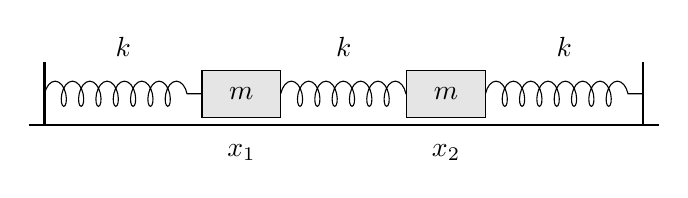
\begin{tikzpicture}[scale=1]
  \draw[thick] (0,0) -- (0,0.8);
  \draw[thick] (7.6,0) -- (7.6,0.8);
  \draw[thick] (-0.2,0) -- (7.8,0);
  \draw[decorate,decoration={coil,aspect=0.5,segment length=2.2mm,amplitude=1.6mm}] (0,0.4) -- (2.0,0.4);
  \draw[fill=gray!20] (2.0,0.1) rectangle (3.0,0.7);  \node at (2.5,0.4) {$m$};
  \draw[decorate,decoration={coil,aspect=0.5,segment length=2.2mm,amplitude=1.6mm}] (3.0,0.4) -- (4.6,0.4);
  \draw[fill=gray!20] (4.6,0.1) rectangle (5.6,0.7);  \node at (5.1,0.4) {$m$};
  \draw[decorate,decoration={coil,aspect=0.5,segment length=2.2mm,amplitude=1.6mm}] (5.6,0.4) -- (7.6,0.4);
  \node at (1.0,1.0) {$k$}; \node at (3.8,1.0) {$k$}; \node at (6.6,1.0) {$k$};
  \node at (2.5,-0.35) {$x_1$}; \node at (5.1,-0.35) {$x_2$};
\end{tikzpicture}
\end{center}

\noindent\textbf{Question:} Suppose we have two carts on a smooth track (perhaps
an airtrack), each with mass $m$, and connected by three equal springs with
spring constants $k$. Find the solution (i.e., $x_1(t)$ and $x_2(t)$) with initial conditions
$x_1(0) = 3$ cm, $x_2(0) = 0$, $\dot{x}_1(0) = \dot{x}_2(0) = 0$.
Here $x_1$ and $x_2$ are each cart's displacement from its own
equilibrium position, with positive $x$ to the right.

\medskip

\noindent\textbf{Step 1: draw the picture, write down N2L.} Cart 1 feels
the left spring, stretched by $x_1$, pulling it back, and the middle
spring, stretched by $x_2 - x_1$, pulling it forward:
\begin{align}
  m\ddot{x}_1 &= -kx_1 + k(x_2 - x_1) = -2kx_1 + kx_2 \label{eq:n2l1} \\
  m\ddot{x}_2 &= -2kx_2 + kx_1 \label{eq:n2l2}
\end{align}

\noindent (We get the second line by symmetry, just swapping the labels.
Look at the signs: a cart's own displacement is opposed by both springs
attached to it, which is the $-2kx_1$ in cart 1's equation; moving the
\emph{other} cart to the right stretches the middle spring, which pulls
this cart to the right too, which is the $+kx_2$. In a moment those become
the negative diagonal and positive off-diagonal entries of a matrix.)

\medskip

\noindent\textbf{Step 2: turn it into a matrix equation.} Writing
$\wo^2 \equiv k/m$,
\begin{equation}
  \label{eq:matrix}
  \begin{pmatrix} \ddot{x}_1 \\ \ddot{x}_2 \end{pmatrix}
  = \wo^2 \begin{pmatrix} -2 & 1 \\ 1 & -2 \end{pmatrix}
  \begin{pmatrix} x_1 \\ x_2 \end{pmatrix},
  \qquad \textrm{i.e.}\qquad \ddot{\vec{x}} = \mathbf{M}\vec{x}.
\end{equation}

The column is the \emph{state} of the system (where both carts are), and
$\mathbf{M}$ is a transformation acting on it. Intuitively, equations
\eqref{eq:n2l1} and \eqref{eq:n2l2} just \textit{look} like a matrix. More
formally, we note that the state we are transforming needs more than one number,
and each derivative is a linear combination of those numbers.

\medskip

\noindent\textbf{Step 3: find the eigenvalues and eigenvectors of
$\mathbf{M}$.} Both methods below start here, so let's get it out of the
way. By definition $\mathbf{M}\vec{v} = \lambda\vec{v}$, so if we plug in
$\vec{v}$, the right-hand side will simplify greatly. Let's see it in
action. To find $\lambda$ we need $\det(\mathbf{M} - \lambda\mathbf{I}) =
0$. We talked extensively in class about how this relates to linear
dependence. We'll find $\lambda$ and
$\vec{v}$ for $\left(\begin{smallmatrix} -2 & 1 \\ 1 & -2
\end{smallmatrix}\right)$, knowing we can multiply by $\wo^2$ at the end
(if $\mathbf{N}\vec{v} = \lambda\vec{v}$ then $(\wo^2\mathbf{N})\vec{v} =
\wo^2\lambda\vec{v}$: same eigenvectors, and the eigenvalues just pick up
the factor):
\begin{equation}
  \begin{aligned}
    \begin{vmatrix} -2-\lambda & 1 \\ 1 & -2-\lambda \end{vmatrix}
    &= (-2-\lambda)^2 - 1 = \lambda^2 + 4\lambda + 3 = (\lambda+1)(\lambda+3) = 0 \\
    &\Rightarrow\quad \lambda \in \{-1, -3\}.
  \end{aligned}
\end{equation}

Now find the eigenvectors: $(\mathbf{M} - \lambda\mathbf{I})\vec{v} = 0$
says
\begin{equation}
  \label{eq:rows}
  \begin{pmatrix} -2-\lambda & 1 \\ 1 & -2-\lambda \end{pmatrix}
  \begin{pmatrix} x_1 \\ x_2 \end{pmatrix}
  = \begin{pmatrix} 0 \\ 0 \end{pmatrix},
  \qquad\textrm{i.e.}\qquad
  \begin{aligned}
    (-2-\lambda)x_1 + x_2 &= 0 \\
    x_1 + (-2-\lambda)x_2 &= 0 .
  \end{aligned}
\end{equation}
Plug $\lambda = -1$ into both rows: $-x_1 + x_2 = 0$ and $x_1 - x_2 = 0$.
The two rows say the same thing, as they must when the determinant is
zero (that is exactly what $\det = 0$ buys you; if the rows disagreed,
you'd have the wrong $\lambda$). So $x_2 = x_1$: only the ratio is fixed,
and we choose $x_1 = 1$, or $\vec{v}_1 = \left(\begin{smallmatrix} 1
\\ 1 \end{smallmatrix}\right)$. Any multiple of an eigenvector is an
eigenvector, so we could have picked $\left(\begin{smallmatrix} 2 \\ 2
\end{smallmatrix}\right)$, etc. Plug $\lambda = -3$ into both rows: $x_1 +
x_2 = 0$ twice, so $\vec{v}_2 = \left(\begin{smallmatrix} 1 \\ -1
\end{smallmatrix}\right)$. Putting the $\wo^2$ back,
\begin{equation}
  \label{eq:eigen}
  \boxed{\;\vec{v}_1 = \begin{pmatrix} 1 \\ 1 \end{pmatrix},\ \lambda_1 = -\wo^2;
  \qquad
  \vec{v}_2 = \begin{pmatrix} 1 \\ -1 \end{pmatrix},\ \lambda_2 = -3\wo^2.\;}
\end{equation}

When we interpret this, we say ``the eigenvalue is $-\omega^2$.'' Felder
and Felder (p.~340) offer ``the resonant frequencies of coupled
oscillators are the square roots of the absolute values of the
eigenvalues'' as a tidbit worth keeping, and it is right here. But don't
drop the sign: the rule works only because the eigenvalues are negative.
The minus sign is the physics: a negative eigenvalue means oscillation; a
positive one would mean exponential growth, and ``the square root of its
absolute value'' would be a frequency for something that doesn't oscillate
at all.

\newpage
\section{The first way: plug in one eigenvector at a time}
\label{sec:way1}

\begin{equation*}
  \boxed{\;\vec{v}_1 = \begin{pmatrix} 1 \\ 1 \end{pmatrix},\ \lambda_1 = -\wo^2;
  \qquad
  \vec{v}_2 = \begin{pmatrix} 1 \\ -1 \end{pmatrix},\ \lambda_2 = -3\wo^2.\;}
  \tag{\ref*{eq:eigen}}
\end{equation*}

\medskip

\noindent\textbf{Each eigenvector becomes a normal mode.} The first
eigenvector tells us that if you plug in \emph{any} state in which $x_2 =
x_1$, the matrix will simply multiply that state by $-\wo^2$. Now, let's
plug in. That means $x_1 = x_2$ at every time (so $\ddot{x}_2 = \ddot{x}_1$
as well), and Equation \eqref{eq:matrix} becomes

\begin{equation}
  \begin{pmatrix} \ddot{x}_1 \\ \ddot{x}_2 \end{pmatrix}
  = \wo^2 \begin{pmatrix} -2 & 1 \\ 1 & -2 \end{pmatrix}
  \begin{pmatrix} x_1 \\ x_2 \end{pmatrix}
  \quad\rightarrow\quad
  \begin{pmatrix} \ddot{x}_1 \\ \ddot{x}_1 \end{pmatrix}
  = \wo^2 \begin{pmatrix} -2 & 1 \\ 1 & -2 \end{pmatrix}
  \begin{pmatrix} x_1 \\ x_1 \end{pmatrix} .
\end{equation}

\noindent And now we use $\mathbf{M}\vec{v} = \lambda\vec{v}$: the column
on the right is a multiple of the eigenvector $\vec{v}_1$, so $\mathbf{M}$
acting on it is just $\lambda_1 = -\wo^2$ times it, and we get

\begin{equation}
  \begin{array}{cccccc}
    & \begin{pmatrix} \ddot{x}_1 \\ \ddot{x}_1 \end{pmatrix}
    & = & \wo^2 & \begin{pmatrix} -2 & 1 \\ 1 & -2 \end{pmatrix}
    & \begin{pmatrix} x_1 \\ x_1 \end{pmatrix} \\[1.5ex]
    & & = & & \mathbf{M} & \vec{v} \\[1.5ex]
    & & = & & \lambda & \vec{v} \\[1.5ex]
    & & = & \wo^2 & (-1) & \begin{pmatrix} x_1 \\ x_1 \end{pmatrix} \\[1.5ex]
    \rightarrow & \ddot{x}_1 & = & & -\wo^2 & x_1
  \end{array}
\end{equation}
(In fact we have this same equation $\ddot{x}_1 = -\wo^2 x_1$ twice.) The matrix multiplication
became a scalar multiplication. That we know how to solve, and the
solution is the first normal mode:
\begin{equation}
  x_1(t) = A_1\cos\wo t + A_2\sin\wo t, \qquad x_2(t) = x_1(t).
\end{equation}

Now the other eigenvector, $x_2 = -x_1$. The same steps, with
$\left(\begin{smallmatrix} -2 & 1 \\ 1 & -2 \end{smallmatrix}\right)
\left(\begin{smallmatrix} x_1 \\ -x_1 \end{smallmatrix}\right) =
(-3)\left(\begin{smallmatrix} x_1 \\ -x_1 \end{smallmatrix}\right)$:
\begin{eqnarray}
  \begin{pmatrix} \ddot{x}_1 \\ -\ddot{x}_1 \end{pmatrix}
  = -3\wo^2 \begin{pmatrix} x_1 \\ -x_1 \end{pmatrix}
  &\rightarrow& \ddot{x}_1 = -3\wo^2 x_1, \quad x_2 = -x_1 \notag \\
  &\rightarrow&
  x_1(t) = B_1\cos\sqrt{3}\,\wo t + B_2\sin\sqrt{3}\,\wo t, \quad x_2(t) = -x_1(t).
\end{eqnarray}

Cool! That's the $\sqrt{3}$ we pulled out of a \textit{hat} back when we first met these
carts.\footnote{Try replacing the state with something that isn't a normal mode,
say $x_2 = 3x_1$: the two rows give you two contradictory differential
equations. Only the eigenvectors work!}

\medskip

\noindent\textbf{The general solution is the sum of the two normal
modes.} Why are we allowed to add them? Equation \eqref{eq:matrix} is
linear, so if two motions solve it, their sum does too (superposition),
even though the sum is no longer a multiple of either eigenvector. Two
second-order equations need four constants, and the sum has exactly four:
\begin{eqnarray}
  \label{eq:foursum}
  x_1(t) &=& A_1\cos\wo t + A_2\sin\wo t + B_1\cos\sqrt{3}\,\wo t + B_2\sin\sqrt{3}\,\wo t \\
  x_2(t) &=& A_1\cos\wo t + A_2\sin\wo t - B_1\cos\sqrt{3}\,\wo t - B_2\sin\sqrt{3}\,\wo t . \notag
\end{eqnarray}
Now we apply our initial conditions. Differentiate and set $t = 0$:
$\dot{x}_1(0) = \wo A_2 + \sqrt{3}\,\wo B_2 = 0$ and $\dot{x}_2(0) = \wo
A_2 - \sqrt{3}\,\wo B_2 = 0$, so $A_2 = B_2 = 0$. We discard the sine
terms, and we're left with
\begin{eqnarray}
  \label{eq:sum}
  x_1(t) &=& A_1\cos\wo t + B_1\cos\sqrt{3}\,\wo t \\
  x_2(t) &=& A_1\cos\wo t - B_1\cos\sqrt{3}\,\wo t . \notag
\end{eqnarray}

\medskip

\noindent\textbf{Let's now be a little clever!}
\begin{equation}
  \label{eq:P}
  \lmat{A_1}{B_1}{x_1(0)}{x_2(0)}{1}{1}{1}{-1}
\end{equation}

\noindent is the matrix that converts normal-mode amplitudes into initial
positions. We can tell that from the column labels, and apparently it's a
matrix of eigenvectors. Why? Well,
\begin{equation}
  \begin{aligned}
    x_1 &= \overbrace{A_1\cos\wo t}^{\text{normal mode 1}}
        &&+ \overbrace{B_1\cos\sqrt{3}\,\wo t}^{\text{normal mode 2}} \\
    x_2 &= A_1\cos\wo t &&- B_1\cos\sqrt{3}\,\wo t
  \end{aligned}
\end{equation}

\noindent Now plug in $t = 0$. The cosines are all $1$, and we get

\begin{equation}
  \begin{pmatrix} x_1(0) \\ x_2(0) \end{pmatrix}
  = \begin{pmatrix} A_1 + B_1 \\ A_1 - B_1 \end{pmatrix}
  = \begin{pmatrix} 1 & 1 \\ 1 & -1 \end{pmatrix}
  \begin{pmatrix} A_1 \\ B_1 \end{pmatrix}.
\end{equation}

\noindent Each column is one normal mode at $t = 0$, which is an
eigenvector. Cool. So, the matrix that converts normal-mode amplitudes to
positions is the matrix of eigenvectors, and the matrix that converts
positions to amplitudes is its inverse, with the labels swapped:
\begin{equation}
  \begin{pmatrix} 1 & 1 \\ 1 & -1 \end{pmatrix}^{-1}
  = \frac{1}{ad - bc}\begin{pmatrix} d & -b \\ -c & a \end{pmatrix}
  = \frac{1}{-2}\begin{pmatrix} -1 & -1 \\ -1 & 1 \end{pmatrix}
  = \begin{pmatrix} 1/2 & 1/2 \\ 1/2 & -1/2 \end{pmatrix}.
\end{equation}
With its labels, which are those of \eqref{eq:P} swapped,
\begin{equation*}
  \lmat{x_1(0)}{x_2(0)}{A_1}{B_1}{1/2}{1/2}{1/2}{-1/2}
\end{equation*}
converts initial conditions to normal-mode amplitudes. Applying it to
ours,
\begin{equation}
  \begin{pmatrix} A_1 \\ B_1 \end{pmatrix}
  = \begin{pmatrix} 1/2 & 1/2 \\ 1/2 & -1/2 \end{pmatrix}
  \begin{pmatrix} 3 \\ 0 \end{pmatrix}
  = \begin{pmatrix} 3/2 \\ 3/2 \end{pmatrix},
\end{equation}

\noindent and the solution is

\begin{equation}
  \label{eq:answer}
  \boxed{\;x_1(t) = \tfrac{3}{2}\cos\wo t + \tfrac{3}{2}\cos\sqrt{3}\,\wo t,
  \qquad
  x_2(t) = \tfrac{3}{2}\cos\wo t - \tfrac{3}{2}\cos\sqrt{3}\,\wo t\;}
\end{equation}

\noindent in cm, with $\wo = \sqrt{k/m}$. \textbf{Whew}!

Check it at $t = 0$: $x_1 = 3$, $x_2 = 0$. Good. Pulling one cart and
holding the other at rest is half of each normal mode, so each cart
carries both frequencies, $\wo$ and $\sqrt{3}\,\wo$. Their periods are in
the ratio $\sqrt{3}$, whatever $k$ and $m$ are. And since two cosines
with frequencies in an irrational ratio never line up again, the motion
never exactly repeats. That's the ``janky''\footnote{I will defend this as a
  technical term to my death.} run we saw on the track.

One caution: the matrix in \eqref{eq:P} is the matrix of eigenvectors
\emph{only at $t = 0$}. At a general $t$ the matrix between
$(A_1, B_1)$ and $(x_1, x_2)$ is
\begin{equation*}
  \lmat{A_1}{B_1}{x_1(t)}{x_2(t)}{\cos\wo t}{\cos\sqrt{3}\,\wo t}{\cos\wo t}{-\cos\sqrt{3}\,\wo t}.
\end{equation*}
Setting $t = 0$ is what turned it into $\left(\begin{smallmatrix} 1 & 1
\\ 1 & -1 \end{smallmatrix}\right)$.\footnote{Is the general-$t$ matrix
always a scalar multiple of $\left(\begin{smallmatrix} 1 & 1 \\ 1 & -1
\end{smallmatrix}\right)$? No. It is the eigenvector matrix times a
diagonal matrix of the two mode factors,
\begin{equation*}
  \begin{pmatrix} \cos\wo t & \cos\sqrt{3}\,\wo t \\ \cos\wo t & -\cos\sqrt{3}\,\wo t \end{pmatrix}
  = \begin{pmatrix} 1 & 1 \\ 1 & -1 \end{pmatrix}
  \begin{pmatrix} \cos\wo t & 0 \\ 0 & \cos\sqrt{3}\,\wo t \end{pmatrix}.
\end{equation*}
Each column is still a multiple of its eigenvector (column 1 is $\vec{v}_1$
times $\cos\wo t$, column 2 is $\vec{v}_2$ times $\cos\sqrt{3}\,\wo t$),
but the two columns are scaled by different amounts, so the whole matrix
is a multiple of $\left(\begin{smallmatrix} 1 & 1 \\ 1 & -1
\end{smallmatrix}\right)$ only when the two cosines are equal: at $t = 0$,
and at isolated later instants, never over an interval, because the two
frequencies differ. Two consequences: first, whenever either cosine is
zero the determinant $-2\cos\wo t\cos\sqrt{3}\,\wo t$ vanishes, so at
those instants you cannot recover the amplitudes from the positions alone
(at every other instant you can, but the matrix you invert is not the
eigenvector matrix; it equals that only at $t = 0$, where both cosines are
$1$). Second, the
factorization is the whole story of the ``better'' way in
\S\ref{sec:way2}: start in amplitude coordinates, let each mode evolve by
its own scalar factor (the diagonal matrix), then convert to positions
with the eigenvector matrix.}

\newpage
\section{The ``better'' way: the natural basis}
\label{sec:way2}

\begin{equation*}
  \boxed{\;\vec{v}_1 = \begin{pmatrix} 1 \\ 1 \end{pmatrix},\ \lambda_1 = -\wo^2;
  \qquad
  \vec{v}_2 = \begin{pmatrix} 1 \\ -1 \end{pmatrix},\ \lambda_2 = -3\wo^2.\;}
  \tag{\ref*{eq:eigen}}
\end{equation*}

\medskip

\noindent This way gets the same answer, but it shows what ``basis'' and
``diagonalization'' mean more directly~\ldots\ and it generalizes super well, as
we'll see. Above, we plugged the eigenvectors in one at a time and watched
what they did to the equation. Instead, let's rewrite the \emph{entire}
equation in the basis defined by the eigenvectors.

\medskip

\noindent\textbf{Question:} Find the general solution to the same
equations, the carts with equal masses $m$,
\begin{equation*}
  \begin{pmatrix} \ddot{x}_1 \\ \ddot{x}_2 \end{pmatrix}
  = \wo^2 \begin{pmatrix} -2 & 1 \\ 1 & -2 \end{pmatrix}
  \begin{pmatrix} x_1 \\ x_2 \end{pmatrix}.
\end{equation*}

\noindent\textbf{Answer:} The eigenvectors of this transformation matrix
are $\left(\begin{smallmatrix} 1 \\ 1 \end{smallmatrix}\right)$ and
$\left(\begin{smallmatrix} 1 \\ -1 \end{smallmatrix}\right)$, with
corresponding eigenvalues $-\wo^2$ and $-3\wo^2$ (boxed above). So, we
can write $x_1$ and $x_2$ in this basis as

\begin{equation}
  \label{eq:fg}
  \begin{pmatrix} x_1(t) \\ x_2(t) \end{pmatrix}
  = f(t)\begin{pmatrix} 1 \\ 1 \end{pmatrix} + g(t)\begin{pmatrix} 1 \\ -1 \end{pmatrix}.
\end{equation}

This says ``you can express the vector $\left(\begin{smallmatrix} x_1 \\
x_2 \end{smallmatrix}\right)$ at any given time as a
linear combination of these two basis vectors, with $f$ and $g$ as the
coefficients'': $f$ is how much of the first normal mode we have, $g$ how
much of the second. This changes in time, so $f$ and $g$ are functions of
$t$. Instead of asking ``where is each cart?'' we are asking ``how much of
each normal mode do we have?''

Can we do that? Yes, for absolutely any functions $x_1$ and $x_2$, and
not because $\vec{v}_1$ and $\vec{v}_2$ are eigenvectors: any two
non-parallel vectors form a basis, so any vector is some combination of
them. That's Section 6.4. Though our life will certainly be better here using an eigenbasis.

What happens when we do that? When we express all our states in a
different basis, the entire equation changes, including the
transformation matrix itself. We'd like to write a corresponding equation
to \eqref{eq:matrix} in this basis:
\begin{equation}
  \label{eq:abcd}
  \begin{pmatrix} \ddot{f} \\ \ddot{g} \end{pmatrix}
  = \begin{pmatrix} a & b \\ c & d \end{pmatrix}
  \begin{pmatrix} f \\ g \end{pmatrix},
\end{equation}

\noindent and we need to know what $a$, $b$, $c$, $d$ are. Two key points
from linear algebra:

\begin{enumerate}
\item[1.] When you use the eigenvectors as a basis, the transformation is
  represented by a diagonal matrix of the eigenvalues. Let's write this
  out: call the eigenvectors $\vec{v}_1$, $\vec{v}_2$ with corresponding
  eigenvalues $\lambda_1$, $\lambda_2$, and take any vector $\vec{v} =
  \alpha\vec{v}_1 + \beta\vec{v}_2$. Apply the transformation; call it
  $\mathbf{T}$, since this works for any matrix (ours is $\mathbf{M}$):
  \begin{equation*}
    \mathbf{T}\vec{v} = \mathbf{T}(\alpha\vec{v}_1 + \beta\vec{v}_2)
    = \alpha\,\mathbf{T}\vec{v}_1 + \beta\,\mathbf{T}\vec{v}_2
    = \alpha\lambda_1\vec{v}_1 + \beta\lambda_2\vec{v}_2 .
  \end{equation*}
  Now read that in the $\{\vec{v}_1, \vec{v}_2\}$ basis. The input coordinates
  are $\left(\begin{smallmatrix} \alpha \\ \beta \end{smallmatrix}\right)$. The
  output is $\left(\begin{smallmatrix} \lambda_1 \alpha \\ \lambda_2 \beta
  \end{smallmatrix}\right)$. So
  \begin{equation*}
    \mathbf{T} = \begin{pmatrix} \lambda_1 & 0 \\ 0 & \lambda_2 \end{pmatrix}
  \end{equation*}
  in this basis: the $a$, $b$, $c$, $d$ of \eqref{eq:abcd} are $\lambda_1$,
  $0$, $0$, $\lambda_2$. (\S\ref{sec:diagonal} says the same thing more
  slowly.)
\item[2.] This naturally decouples our equations.
\end{enumerate}

\noindent We can immediately write it. In the eigenvector basis,
\eqref{eq:matrix} becomes

\begin{equation}
  \label{eq:diag}
  \begin{pmatrix} \ddot{f} \\ \ddot{g} \end{pmatrix}
  = \begin{pmatrix} -\wo^2 & 0 \\ 0 & -3\wo^2 \end{pmatrix}
  \begin{pmatrix} f \\ g \end{pmatrix}
  \qquad\Rightarrow\qquad
  \ddot{f} = -\wo^2 f, \quad \ddot{g} = -3\wo^2 g .
\end{equation}

The natural basis has done its job. Those are two separate simple
harmonic oscillators, so

\begin{equation}
  f = A_1\cos\wo t + A_2\sin\wo t, \qquad g = B_1\cos\sqrt{3}\,\wo t + B_2\sin\sqrt{3}\,\wo t .
\end{equation}

Finally, we go back to our position basis $(x_1, x_2)$ with
\eqref{eq:fg}, $x_1 = f + g$ and $x_2 = f - g$:
\begin{equation}
  \boxed{\;
  \begin{aligned}
    x_1 = f + g &= A_1\cos\wo t + A_2\sin\wo t + B_1\cos\sqrt{3}\,\wo t + B_2\sin\sqrt{3}\,\wo t \\
    x_2 = f - g &= A_1\cos\wo t + A_2\sin\wo t - B_1\cos\sqrt{3}\,\wo t - B_2\sin\sqrt{3}\,\wo t
  \end{aligned}\;}
\end{equation}

So, four constants, as there must be, and it is exactly
\eqref{eq:foursum}: the same answer as the first way.

\medskip

\noindent\textbf{The initial conditions, this way.} Solving
\eqref{eq:fg} for the coefficients gives $f = (x_1 + x_2)/2$ and $g =
(x_1 - x_2)/2$ (that's the inverse matrix from \S\ref{sec:way1} again,
read as two equations). For $x_1(0) = 3$, $x_2(0) = 0$ that's $f(0) =
g(0) = 3/2$: the same amplitudes, and the same solution
\eqref{eq:answer}. Physically, $f$ is how far the midpoint of the two carts
has moved from equilibrium, and
$g$ is half the compression of the middle spring, which is a nice way to see
why the slow mode never stretches the middle spring and the fast one
stretches it twice as much as either cart moves.

\section{Why is the matrix diagonal in the eigenvector basis?}
\label{sec:diagonal}

Before we dive into the eigenproblem, let's review some general
change-of-basis thoughts. The basis we're used to working with is the
$\{\hat{\imath}, \hat{\jmath}\}$ basis: $\hat{\imath} =
\left(\begin{smallmatrix} 1 \\ 0 \end{smallmatrix}\right)$, $\hat{\jmath} =
\left(\begin{smallmatrix} 0 \\ 1 \end{smallmatrix}\right)$. Let's pick
another basis to consider, say $\vec{v}_1 = \hat{\imath} + \hat{\jmath}$ and
$\vec{v}_2 = -3\hat{\imath} + 4\hat{\jmath}$. Then what we want is some
matrix
\begin{equation*}
  \lmat{\vec{v}_1}{\vec{v}_2}{\hat{\imath}}{\hat{\jmath}}{\phantom{-3}}{\phantom{-3}}{\phantom{-3}}{\phantom{-3}}
\end{equation*}
to turn $\{\hat{\imath}, \hat{\jmath}\}$ into $\{\vec{v}_1, \vec{v}_2\}$.
The easy matrix to write down is
\begin{equation*}
  \lmat{\vec{v}_1}{\vec{v}_2}{\hat{\imath}}{\hat{\jmath}}{1}{-3}{1}{4}
\end{equation*}
whose columns are just $\vec{v}_1$ and $\vec{v}_2$. But look at the
labels: this is a matrix that eats a pair of $\{\vec{v}_1, \vec{v}_2\}$
amplitudes and spits out $\{\hat{\imath}, \hat{\jmath}\}$ amplitudes.
(Feed it $\left(\begin{smallmatrix} 1 \\ 0 \end{smallmatrix}\right)$,
meaning one $\vec{v}_1$ and no $\vec{v}_2$, and out comes
$\left(\begin{smallmatrix} 1 \\ 1 \end{smallmatrix}\right)$, which is
$\vec{v}_1$ in $\hat{\imath}, \hat{\jmath}$ components.) That's the
opposite of what we asked for. Its inverse,
\begin{equation*}
  \begin{pmatrix} 1 & -3 \\ 1 & 4 \end{pmatrix}^{-1}
  = \frac{1}{7}\begin{pmatrix} 4 & 3 \\ -1 & 1 \end{pmatrix},
\end{equation*}
does the opposite, which is the thing we wanted. Let's check:
$\left(\begin{smallmatrix} 2 \\ 3 \end{smallmatrix}\right)$ in
$\{\hat{\imath}, \hat{\jmath}\}$ should go to some pair of
$\{\vec{v}_1, \vec{v}_2\}$ amplitudes:
\begin{equation*}
  \frac{1}{7}\begin{pmatrix} 4 & 3 \\ -1 & 1 \end{pmatrix}
  \begin{pmatrix} 2 \\ 3 \end{pmatrix}
  = \frac{1}{7}\begin{pmatrix} 8 + 9 \\ -2 + 3 \end{pmatrix}
  = \begin{pmatrix} 17/7 \\ 1/7 \end{pmatrix},
\end{equation*}
and then
\begin{equation*}
  \frac{17}{7}\begin{pmatrix} 1 \\ 1 \end{pmatrix}
  + \frac{1}{7}\begin{pmatrix} -3 \\ 4 \end{pmatrix}
  = \begin{pmatrix} (17 - 3)/7 \\ (17 + 4)/7 \end{pmatrix}
  = \begin{pmatrix} 14/7 \\ 21/7 \end{pmatrix}
  = \begin{pmatrix} 2 \\ 3 \end{pmatrix}. \checkmark
\end{equation*}
So: the matrix whose columns are the new basis vectors is the easy one to
write, and it converts new-basis amplitudes into old-basis components.
Going the other way costs an inverse. That's exactly what happened with
$\mathbf{P}$ in \S\ref{sec:way1}.

\medskip

\noindent Now back to the eigenproblem. Felder and Felder say ``This fact comes very directly from the definition
of an eigenvector'' and leave it there (p.\ 339; it's their Problem
6.206). We wrote it out under key point 1 in \S\ref{sec:way2}; here it
is again, more slowly. The only facts we need are that matrix
multiplication is linear, the definition $\mathbf{T}\vec{v}_i =
\lambda_i\vec{v}_i$, and that $\vec{v}_1$ and $\vec{v}_2$ are independent,
so they form a basis (true here, since the eigenvalues differ).

Let $\vec{v}_1$, $\vec{v}_2$ be the eigenvectors of some transformation
$\mathbf{T}$, with eigenvalues $\lambda_1$, $\lambda_2$. Take any vector
and write it in the eigenvector basis:
\begin{equation}
  \vec{v} = \alpha\vec{v}_1 + \beta\vec{v}_2 ,
\end{equation}

\noindent so $\vec{v}$ has coordinates $(\alpha, \beta)$ in the $\{\vec{v}_1, \vec{v}_2\}$
basis. Apply $\mathbf{T}$. It acts on each piece separately (linearity),
and by the definition of an eigenvector it does nothing to each piece
except scale it:
\begin{equation}
  \mathbf{T}\vec{v} = \mathbf{T}(\alpha\vec{v}_1 + \beta\vec{v}_2)
  = \alpha\,\mathbf{T}\vec{v}_1 + \beta\,\mathbf{T}\vec{v}_2
  = \alpha\lambda_1\vec{v}_1 + \beta\lambda_2\vec{v}_2 .
\end{equation}
Now read that in the $\{\vec{v}_1,\vec{v}_2\}$ basis. The input had coordinates
$\left(\begin{smallmatrix} \alpha \\ \beta \end{smallmatrix}\right)$. The output has
coordinates $\left(\begin{smallmatrix} \lambda_1 \alpha \\ \lambda_2 \beta
\end{smallmatrix}\right)$. The only matrix that takes
$(\alpha, \beta)$ to $(\lambda_1 \alpha, \lambda_2 \beta)$ is

\begin{equation}
  \boxed{\;\mathbf{T} \textrm{ in the } \{\vec{v}_1, \vec{v}_2\} \textrm{ basis}
  = \begin{pmatrix} \lambda_1 & 0 \\ 0 & \lambda_2 \end{pmatrix}\;}
\end{equation}

\noindent That's the whole proof. In the $\{\hat{\imath}, \hat{\jmath}\}$ basis,
$\mathbf{T}$ mixes the components (the off-diagonal entries are nonzero),
because $\hat{\imath}$ and $\hat{\jmath}$ are not eigenvectors. In the
eigenvector basis there is no mixing left to describe. Said another way:
the columns of a matrix are the images of the basis vectors, and the
image of $\vec{v}_1$ is $\lambda_1\vec{v}_1$, which in this basis is
$(\lambda_1, 0)$.

For the springs, replace $\mathbf{T}$ by $\mathbf{M}$ and $\vec{v}$ by the
state: plug \eqref{eq:fg} into \eqref{eq:matrix} to get
$\ddot{f}\vec{v}_1 + \ddot{g}\vec{v}_2 = f\lambda_1\vec{v}_1 +
g\lambda_2\vec{v}_2$, and since $\vec{v}_1$ and $\vec{v}_2$ are
independent, match coefficients: $\ddot{f} = \lambda_1 f$, $\ddot{g} =
\lambda_2 g$. That is \eqref{eq:diag}.

\section{Which way should I use?}
\label{sec:which}

For one $2\times 2$ problem by hand: it doesn't matter. The time-consuming part,
finding the eigenvalues and eigenvectors (the determinant, the quadratic,
two little linear systems), is shared, and neither method avoids it.
After that, the first way substitutes each eigenvector in and fits the
initial conditions with one $2\times 2$ solve; the second way gets the
decoupled equations in one line and fits the initial conditions with the
same $2\times 2$ solve dressed up as an inverse. The first way is a shade
quicker (the substitution doubles as a check that your eigenvector is
right); the second is a shade cleaner. Meh. A wash.

\textbf{However,} once the problem gets bigger (or gets reused), the second way wins:

\begin{itemize}
\item \textbf{Many degrees of freedom.} For $N$ carts, both ways find $N$
  eigenvectors and fit $N$ initial conditions; the second way packages
  all of it as one matrix product. On a computer that is the whole story:
  \texttt{numpy.linalg.eig} once, then, for carts released from rest,
  $\vec{x}(t) = \mathbf{P}\,\mathrm{diag}(\cos\omega_i t)\,\mathbf{P}^{-1}\vec{x}(0)$,
  where $\mathbf{P}$ is the matrix of eigenvectors as columns (the matrix
  in \eqref{eq:P}) and $\omega_i = \sqrt{-\lambda_i}$: one line for any
  $N$. (Nonzero initial velocities add a second term of the same shape,
  with $\sin(\omega_i t)/\omega_i$ in place of $\cos\omega_i t$ and
  $\dot{\vec{x}}(0)$ in place of $\vec{x}(0)$.)
\item \textbf{Reuse.} A driving force, or damping that is the same on every
  cart, leaves the eigenvectors alone. The second way then just adds a
  term to each one-dimensional equation; the first way has to redo the
  substitution. (New initial conditions cost the same either way: one
  $2\times 2$ solve.)
\item \textbf{Understanding.} The second way is the one that says
  \emph{why} only those two ratios work: only in the basis of the normal
  modes does the matrix become diagonal; no other basis decouples the
  equations.
\end{itemize}

Felder and Felder (p.~340) put it this way. In both approaches the
takeaway is ``the eigenvectors of the matrix define the normal modes of
the system.'' The second approach ``is less direct, but it gives you
perhaps the clearest view of why these normal modes work and no others
would.'' My own one-line version: the first way is how you compute a
given problem; the second is why the computation works. And their advice:
``If you find the
second approach confusing start by getting comfortable with the first
approach \ldots\ but once you have worked with it a while come back to
the second approach and see if you can see how it is doing the same thing
as the first one, but in a different basis.''

\section{The general procedure, and the unequal-mass carts}
\label{sec:procedure}

Now for the capstone problem: you have the carts at the front of the room. And
you can add masses to each of them. Your goal is to pick a set of masses, to
predict the normal modes, and then to physically test it all out. To be clear,
the three springs have equal spring constants $k$, but now your carts will have
different masses. The general procedure is:

\begin{enumerate}
\item[1.] Draw the picture.
\item[2.] Write down N2L for each cart.
\item[3.] Turn it into a matrix equation $\ddot{\vec{x}} = \mathbf{M}\vec{x}$.
\item[4.] Find the normal modes: the eigenvectors of $\mathbf{M}$ give the
  ratio of $x_2$ to $x_1$ in each mode, and the eigenvalues give
  $-\omega^2$.
\item[5.] Combine them (either way) and use the initial conditions.
\end{enumerate}

\noindent You can just jump in. If you want a small hint, here's how I dealt
with notation: For different masses $m_1$ and $m_2$, it's convenient to just
think about which mass is bigger and by how much. So, call the mass ratio $\mu =
m_1/m_2$. Then, once you've gotten $\mathbf{M}$, you can pull out a $k/m_1$ so
that it just looks like constants and $\mu$.

\medskip

\noindent\textbf{Choosing your masses.} Decide which cart is cart 1
before you write N2L (swapping the labels sends $\mu$ to $1/\mu$), and make
the heavier cart about one and a half to three times the lighter one. Much
closer to equal and the carts behave like the equal-mass case you've
already solved. Much more unequal and the modes separate into ``the light
cart bounces while the heavy one barely moves'' and ``the heavy cart drags
the light one along,'' which is easy to produce but hard to judge: almost
any pluck of the light cart will look like a clean mode, because the heavy
cart's response is too small to see.

\medskip

\noindent\textbf{How to tell you've isolated a mode.} In a normal mode both
carts turn around at the same instants, keep a fixed ratio of amplitudes,
and nothing changes from cycle to cycle. If you missed, the energy sloshes:
one cart's swing shrinks while the other's grows, and for a moment one cart
sits nearly still while the other moves. Predict, before you touch the
track, the sign of $x_2/x_1$ in each mode, roughly how big it is, and how
many fast cycles fit in one slow cycle; then count, don't time.


\newpage
Here's my solution: step 2 gives $m_1\ddot{x}_1 = -2kx_1 + kx_2$ and
$m_2\ddot{x}_2 = kx_1 - 2kx_2$. Divide each line by its own mass:
\begin{alignat*}{3}
  \ddot{x}_1 &={}& -2\frac{k}{m_1}x_1 && {}+\frac{k}{m_1}x_2 \\
  \ddot{x}_2 &={}& \frac{k}{m_2}x_1 && {}-2\frac{k}{m_2}x_2
\end{alignat*}
which is already shaped like a matrix equation. Now put in $\mu$: since
$k/m_2 = \mu\,(k/m_1)$,
\begin{alignat*}{3}
  \ddot{x}_1 &={}& -2\frac{k}{m_1}x_1 && {}+\frac{k}{m_1}x_2 \\
  \ddot{x}_2 &={}& \mu\frac{k}{m_1}x_1 && {}-2\mu\frac{k}{m_1}x_2
\end{alignat*}
and pulling the common $k/m_1$ out front,
\begin{equation}
  \mathbf{M} = \frac{k}{m_1}\begin{pmatrix} -2 & 1 \\ \mu & -2\mu \end{pmatrix}.
\end{equation}
Plug in your $\mu$ and do step 4.

You will find that the eigenvectors are no longer
$\left(\begin{smallmatrix} 1 \\ 1 \end{smallmatrix}\right)$ and
$\left(\begin{smallmatrix} 1 \\ -1 \end{smallmatrix}\right)$. Writing $s =
\sqrt{\mu^2 - \mu + 1}$ for short, the eigenvectors are
\begin{equation}
  \label{eq:unequal}
  \vec{v}_{\rm slow} = \begin{pmatrix} 1 \\ 1 - \mu + s \end{pmatrix}
  \qquad\text{and}\qquad
  \vec{v}_{\rm fast} = \begin{pmatrix} 1 \\ 1 - \mu - s \end{pmatrix},
\end{equation}
with corresponding eigenvalues
\begin{equation}
  \label{eq:unequal-lambda}
  \lambda_{\rm slow} = \frac{k}{m_1}\bigl(-(1+\mu) + s\bigr)
  \qquad\text{and}\qquad
  \lambda_{\rm fast} = \frac{k}{m_1}\bigl(-(1+\mu) - s\bigr).
\end{equation}
(Check: $\mu = 1$ gives $s = 1$, so $\lambda = -k/m_1$ and $-3k/m_1$ with
$x_2/x_1 = \pm 1$, as in (\ref*{eq:eigen}).) The heavier cart moves more
in the slow mode and less in the fast one. The ratio of the two periods
should turn out to be $T_{\rm slow}/T_{\rm fast} =
\sqrt{\lambda_{\rm fast}/\lambda_{\rm slow}}$.

\medskip


\end{document}
